% original by Dr Kelly Homan

% hosted project:
% http://code.google.com/p/missouri-science-technology-latex-dissertation-thesis-template/

% email list:
% S&T Thesis/Dissertation LaTeX Template User Group <latextdt-grp@mst.edu>

% google group:
% https://groups.google.com/a/mst.edu/group/latextdt-grp/topics?hl=en

% see http://grad.mst.edu/currentstudents/thesesdissertations/
% for guidelines
\documentclass[times,12pt,titlepage]{mstthesis} % 
\doublespacing
% Dr Parris, Vojta, Story, and Yamilov would prefer single spaced, double sided print
% Binding and printing: 
% Library needs good paper, bound. Department can uses either good or normal paper, also bound. Department will pay for binding of these two copies.
% Dr Yamilov wants two copies on good paper, single spaced and double sided; bound (one for him, one for Hui Cao). Cost of binding is $10 per copy through department. 
% Parents printed copy

% Ben isn't sure what the purpose of the following are
\usepackage{fancyhdr}
\pagestyle{fancy}
\lhead{}\chead{}\rhead{\thepage}
\lfoot{}\cfoot{}\rfoot{}
\renewcommand{\headrulewidth}{0pt}
\renewcommand{\footrulewidth}{0pt}

% Ben's additions
\usepackage{comment} % multi-line comments
\usepackage{graphicx} % necessary for inclusion of .eps for figures

%Find the pictures
\graphicspath{ {./images/} {../images/} }

% the following is for published chapters to note where they were published
\renewcommand{\thefootnote}{\fnsymbol{footnote}}
% http://help-csli.stanford.edu/tex/latex-footnotes.shtml

% Use the first command below if you want captions over 1 line indented. A side
% effect of this is to remove the use of bold for captions. To restore bold,
% also include the second line below.
\usepackage[hang]{caption}  
% change the caption delimiter in caption2.sty from a colon to a period:
%\renewcommand\captionlabeldelim{.}
%\usepackage{hangcaption}

% % \usepackage{algorithmic}
% % \usepackage{algorithm}
% % \usepackage{url}
% % \usepackage{lscape}
% % \usepackage{subfigure}
% % \usepackage{flafter} % http://stackoverflow.com/questions/547508/in-latex-is-there-a-way-to-put-a-float-automatically-after-where-it-is-first-re
% % 
% % 
% % %%\ExecuteOptions{textures}

%\usepackage{titlesec}% http://ctan.org/pkg/titlesec
%\usepackage{lipsum}% http://ctan.org/tex-archive/macros/latex/contrib/lipsum   http://ctan.org/pkg/lipsum

%\usepackage{tocloft} % http://ctan.org/pkg/tocloft

% http://en.wikibooks.org/wiki/LaTeX/Page_Layout#Widows_and_orphans
\widowpenalty=10000 % prevents the first line of a paragraph from being alone at the bottom of a page. It will either cause that line to move to the next page, or cause one line from the next page to join the lone line. 
\clubpenalty=10000  % prevent the last line of a paragraph to be alone at the top of a page. At best it will force there to be two lines. 
% MS&T Office of Grad Studies says ``Need to have at least 2 lines at the top and at the bottom of every page. No lone headers at bottom of page.
% see https://groups.google.com/d/msg/comp.text.tex/uN7tvjubk8o/kcUvevut0hEJ

% brokenpenalty is meant to eliminate hyphenation of words at the end of a page. However, it may introduce non-uniform pages
% https://groups.google.com/d/msg/comp.text.tex/pBSOMuQzOH0/innVfjc3ZG4J
\brokenpenalty=10000 % having this causes page numbers to be incorrect in ToC. Not having it causes word breaks at end of page
% better solution, as per Gerry Howser:
%\raggedbottom
% However, it doesn't fix hyphenation at end of page

% http://en.wikibooks.org/wiki/LaTeX/Formatting#Hyphenation
%\hyphenation{local-ization diff-usion}

%\usepackage{enumerate}

% for T/E paper
%\usepackage{graphicx}
\usepackage{epsfig}
\usepackage{color}
\usepackage{verbatim} % multi-line comments
\usepackage{subfigure}             % allows for use of "sub figure" 1a, 1b, etc

% for D(z) PRB
% % %\usepackage[fleqn]{amsmath}
% % %\usepackage{amsthm}
%\usepackage{amsmath} % adding this doesn't fix the symbol problem, as the package is required by mstthesis.cls
%\usepackage{mathtools} % this 
\usepackage{amssymb} % \gtrsim

\usepackage{makeidx} % Index
\makeindex
%\usepackage{glossary}
\usepackage[xindy,toc]{glossaries} % http://en.wikibooks.org/wiki/LaTeX/Glossary
\makeglossary  % http://texblog.wordpress.com/2007/11/01/glossary-in-latex/

% Note: hyperref must be the last package
\usepackage[breaklinks=true, % allow links to break over lines by making links over multiple lines into PDF links to the same target 
% hyperindex, % Makes the page numbers of index entries into hyperlinks. 
% %backref, 
%pdftex,
%bookmarks=true % bookmark hierarchy is incorrect   http://www.latex-community.org/forum/viewtopic.php?f=47&t=7762
%bookmarksnumbered=true
% %pagebackref, % Adds backlink text to the end of each item in the bibliography, as a list of page numbers. 
linktocpage, % make page number, not text, be link on TOC, LOF and LOT 
% colorlinks=false, 
pdftitle={Dissertation}, 
pdfauthor={Ben Payne}, 
pdfsubject={PhD dissertation}, 
pdfkeywords={exam dissertation anderson localization random media gain}
]{hyperref}

%ps% ... uncomment after editing toc, lof, lot ...
%ps%\nofiles

\begin{document}

%ps% ... specify: ms | phd ...
\begin{ThesisTitlePage}{phd}

\author{\MakeUppercase{Benjamin Henry Payne}}

\thesistitle{SOMETHING SOMETHING GROUP MANAGEMENT}

\department{Computer Science}

\degree{Doctor of Philosophy}

%ps% ... thesis committee ...

\ThesisAdviser{Dr. Bruce McMillin}

%ps% If you have a co-advisor, enter the name in the
%ps% curly braces below and uncomment.
%ps% Otherwise, leave commented out.
%ps%\cothadviser{} % If you have 2 thesis advisers

\memberone{Dr. Alireza Hurson}
\membertwo{Dr. Wei Jiang}
\memberthree{Dr. Sriram Chellappan}
\memberfour{Dr. Sahra Sedighsarvestani}

%ps% ... Graduation date.  NOT your submission date! ...
\graddate{2013}

\end{ThesisTitlePage}

%ps% ... copyright page - true|false ...
% from 
% http://creativecommons.org/choose/

%This work is licensed under the Creative Commons Attribution-NonCommercial-ShareAlike 3.0 Unported License. To view a copy of this license, visit 
%\\\mbox{\href{http://creativecommons.org/licenses/by-nc-sa/3.0/}{http://creativecommons.org/licenses/by-nc-sa/3.0/}} 
%or send a letter to Creative Commons, 444~Castro Street, Suite~900, Mountain View, California, 94041, USA.

%\ \\
%Published journal articles retain their original copyrights.

% http://www.tandf.co.uk/journals/contact.asp
% Customer Services for Taylor & Francis Group Journals
% T&F Customer Services
% 325 Chestnut Street
% Suite 800
% Philadelphia, PA 19106, USA
% 
% http://journalauthors.tandf.co.uk/preparation/copyright.asp
% 
% "the right to include an article in a thesis or dissertation that is
% not to be published commercially, provided that acknowledgement to
% prior publication in the relevant Taylor & Francis journal is made
% explicit;"
% 
% 
% ****************************
% APS Headquarters
% One Physics Ellipse
% College Park, MD 20740-3844
% (301) 209-3200
% 8am-6pm M-F
% 
% http://publish.aps.org/copyrightFAQ.html#thesis
% 
% "As the author of an APS-published article, may I include my article
% or a portion of my article in my thesis or dissertation?"
% 
% "Yes, the author has the right to use the article or a portion of the
% article in a thesis or dissertation without requesting permission from
% APS, provided the bibliographic citation and the APS copyright credit
% line are given on the appropriate pages."
% 
% ****************************
% Elsevier: 1 888 834 7287
% 
% http://www.elsevier.com/wps/find/authorsview.authors/rights
% 
% "the right to include the journal article, in full or in part, in a
% thesis or dissertation;"

\copyrightyear{2013}
\ThesisCopyrightPage{false}

%ps% ... front matter - publication option - ms|phd...

%\begin{ThesisPublicationOption}{phd}
%This dissertation has been prepared in the form of six papers.

%\renewcommand{\theenumi}{Paper \arabic{enumi}}
%\begin{enumerate}%[Paper 1]

%  http://tex.stackexchange.com/questions/38139/how-can-i-calculate-the-difference-of-2-counters-pageref
% \newcounter{tempor}
% \setcounter{tempor}{\pageref{paper:1_start}}
% \addtocounter{tempor}{1}
%\item Pages~\arabic{temp}--\pageref{paper:1_end} have been published as
%\item Pages~\pageref{paper:1_start}--\pageref{paper:1_end} have been published as 
%  \textit{\href{http://link.aps.org/doi/10.1103/PhysRevB.82.104204}{Relation between transmission and energy stored in random media with gain}}, Physical Review B \textbf{82} 104204 (2010) with Jonathan Andreasen, Hui Cao, and Alexey Yamilov.
%\item Pages~\pageref{paper:2_start}--\pageref{paper:2_end} have been published as 
%  \textit{\href{http://dx.doi.org/10.1080/09500340.2010.519443}{Classification of regimes of wave transport in non-conservative random media}}, Journal of Modern Optics (2010) with Alexey Yamilov.
%\end{enumerate}
%\renewcommand{\theenumi}{\arabic{enumi}}

%An earlier letter, 
%\textit{\href{http://dx.doi.org/10.1016/j.physb.2010.01.025}{Criterion for light localization in random amplifying media}}, 
%has been published in Physica B \textbf{405}, 3012--3015 (2010) with Hui Cao and Alexey Yamilov. This is reported in Paper 1.

%\end{ThesisPublicationOption}
%ps% ... front matter - thesis abstract ...
\begin{ThesisAbstract}
\begin{abstract}
Cyber-physical systems (CPS) are an attractive option for future development of
critical infrastructure systems. By supplementing the traditional physical
network with cyber control, the performance and reliability of the system
can be increased. In some of these networks, distributing the cyber control
offers increased redundancy and availability during fault conditions. However,
there are very few works which study the effects of cyber faults on a 
distributed cyber-physical system. These are of a particular interest in the smart grid
environment where outages and failures are very costly. By examining the
behavior of a distributed system under fault scenarios, the overall robustness
of the system can be improved by planning characteristics and responses to
faults that allow the system to continue operating in difficult circumstances.

This work examines the consequences of network unreliability on a core part of the
 Distributed Grid Intelligence (DGI) for the FREEDM (Future Renewable Electric 
Energy Delivery and Management) Project. By applying different rates of packet
loss in specific configurations to the communication stack of the software and
observe the behavior of a critical component (Group Management) under those
conditions. These components identify the amount of time spent in a group,
working, as a function of the network reliability. Given this one can parameterize
the amount of messages that are lost and thus the number of failed physical actuations.
Knowing this and the physical characteristics of the system, one can tune the amount
of time between reconfiguration in order to prevent the number of failed physical
changes from causing the system to become unstable. Using this, we can develop
methods and guarantees to protect the operation of a CPS.
\end{abstract}

\end{ThesisAbstract}

%ps% ... front matter - acknowledgements ...
\begin{ThesisAcknowledgment}
The author acknowledges the support of the Future Renewable
Electric Energy Delivery and Management Center,
a National Science Foundation supported Engineering Research
Center under grant NSF EEC-081212, and the United States Department of Education GAANN program.

\end{ThesisAcknowledgment}

%ps% ... toc, lof, and lot (list of symbols in respective papers) ...
\begin{ThesisFrontMatter}
\tableofcontents
\listoffigures
\listoftables
\end{ThesisFrontMatter}

\newcommand{\boldnabla}{\mbox{\boldmath$\nabla$}}
\newcommand{\boldrho}{\mbox{\boldmath$\rho$}}

%ps% ... chapter 1 - ptointroduction ...
\begin{ThesisBody}
%Here is dissertation body
% Introduce the contents of the paper and what will be presented
\chapter{Introduction}

The design of stochastic models of distributed systems has a long history as a challenging area of interest.
Models of distributed systems have to deal with a number of factors.
These factors include the various types of failure the system could experience, a lack of tightly synchronized execution, and a large complex state space when there are a high number of agents\cite{DISTRIBUTED}\cite{distributed-challenges}. 
However, the concept of distributed systems plays a central role in many of the future visions for how critical infrastructure will operate.
These critical infrastructures are physical networks whose operation are so vital that if those networks failed to operate correctly it would be highly detrimental to the population that rely on those systems.
\ac{CPS} are the integration of computational systems with physical networks.
Computational systems already play a critical role in most critical infrastructures, and as demands for security features, such as accessibility, increase distributed systems are becoming an increasingly favorable choice for the computational needs for these systems\cite{SMARTGRIDBENEFITS}.

The \ac{FREEDM} center\cite{FREEDM}, an NSF funded ERC envisions a future power-grid where widely distributed renewable power generation and storage is closely coupled with a distributed system that facilitates the dispatch of power across those areas.
Other systems like \ac{VANET}\cite{CARS1}\cite{CARS2}\cite{vanet-congestion} and air traffic control systems\cite{AIRTRAFFIC1}\cite{AIRTRAFFIC2} also propose similar control systems where many computers must cooperate to ensure both smooth operation and the safety of the people using those systems.
As a consequence, ensuring that the computer systems that control those infrastructures behave correctly during fault conditions is critical, especially when those computer systems rely on their interaction with other computers to operate.

A robust \ac{CPS} should be able to survive and adapt to communication network outages in both the physical and cyber domains.
When one of these outages occurs, the physical or cyber components must take corrective action to allow the rest of the system to continue operating normally.
Additionally, processes may need to react to the state change of some other process.
Managing and detecting when other processes have failed is commonly handled by a leader election algorithm and failure detector.

In a smart-grid system, misbehavior during fault conditions could lead to critical failures such as a blackout or voltage collapse. In a \ac{VANET} or air traffic control system, vehicles could collide, injuring passengers or destroying property. Additionally, since these systems are a part of critical infrastructure, protecting them from malicious entities is an important consideration.

This work was motivated by observations on the effects of lost messages on the group management module of the \ac{DGI} used by the \ac{FREEDM} smart-grid project.
These original observations confirmed the need to explore more well defined models for the behaviors of \ac{CPS} in order for them to better serve the people that use them.

We present a framework for reasoning about inferable state in the context of a distributed system. To do this, we exploit existing work in the field of information flow security. Information flow security has been used to reason about how attacks like STUXNET can manipulate operators beliefs while disrupting a system\cite{STUXNET}. In particular, these approaches reason about how the operator in a STUXNET attack has no avenue to verify the reports from a compromised computing device. Using existing modal logic frameworks and using information flow security models\cite{Howser2012}\cite{STUXNET}\cite{Howser2013}, one can formally reason about where information that is not normally known to a domain can be inferred.

We will show in this work that in a system with the correct information flows, an agent in a distributed system can infer the state of other agents in the system. With this information, that agent can then construct a reasonable model of the system to determine if the current behavior could lead to an undesirable situation with either the cyber or physical network.

Using this framework we present a leader election algorithm that can be modeled with a Markov chain for a known omission fault\cite{OMISSIONFAILURES} rate.
The presented algorithm maintains the Markov property for the observations of the leader despite omission faults.
This approach to considering how a distributed system interacts during a fault condition allows for the creation of new techniques for managing a fault scenario in cyber-physical systems.
In the context of \ac{FREEDM}, these models produce expectations of how much time the DGI will be able to spend coordinating and doing useful work.
Using these measures, the behavior of the control system for the physical devices can be adjusted to prevent faults, like blackouts and voltage collapse, in the physical network.

We also propose using existing schemes to detect communication network congestion and inform processes in a \ac{CPS} of impending congestion.
Processes act on this information to change their behavior in anticipation of message delays or loss.
This behavior allows them to harden themselves against the congestion, and allows them to continue operating as normally as possible during the congestion.
This technique involves changing the behavior of both the leader election\cite{INVITATIONELECTION} and physical device management algorithm during congestion.

To accomplish this, we extend existing networking concepts of \ac{RED}, \ac{ECN}\cite{RFCECN}, and ICMP source quench\cite{RFCSOURCEQUENCH}.
When a network device detects congestion, it notifies processes that the network is experiencing congestion and they should react appropriately.
We demonstrate an implementation of the \ac{FREEDM} \ac{DGI} in a \ac{NS3} simulation environment\cite{NS3} with our congestion detection feature.
The \ac{DGI} operates normally until the simulation introduces a traffic flow that congests the network devices in the simulation.
After congestion has been identified by the \ac{RED} queuing algorithm, the \ac{DGI} are informed. %via UDP multicast.
When the congestion notifications are introduced, the \ac{DGI} maintains configurations which they would normally be unable to maintain during congestion.
Additionally, we show a greater amount of work can be done without the work causing unstable power settings to be applied.



\chapter{Background Theory}
\section{FREEDM DGI}
The FREEDM DGI is a smart grid operating system that organizes and coordinates 
power electronics and negotiates contracts to deliver power to devices and 
regions that cannot effectively facilitate their own need.

To accomplish this, the DGI software consists of a central component, the 
broker, which is responsible for presenting a communication interface and 
furnishing any common functionality needed by any algorithms used by the 
system. These algorithms are grouped into modules.

The intial work this document uses a version of the FREEDM DGI software with 
only one module: group management. Group management implements a leader
election algorithm to discover which nodes are reachable in the cyber domain.

\section{Broker Architecture}

The DGI software is designed around the broker architecture specification. Each 
core functionality of the system is implemented within a module 
which is provided access to core interfaces which deliver functionality such as 
scheduling requests, message passing, and a framework to manipulate physical 
devices, including those which exist only in simulation environments such as 
PSCAD\cite{PSCAD} and RSCAD\cite{RSCAD}.

The Broker provides a common message passing interface which all modules are 
allowed access to. This interface also provides the inter-module communication 
which delivers messages between software modules, effectively decoupling them 
outside of the requirement for them to be able to recognize messages addressed 
to them from other modules.

Several of the distributed algorithms used in the software require the use of 
ordered communication channels. To achieve this, FREEDM provides a reliable 
ordered communication protocol (The sequenced reliable connection or SRC) to 
the modules, as well as a ``best effort'' protocol (The sequenced unreliable 
connection or SUC) which is also FIFO (first in, first out), but provides 
limited delivery guarantees.

We elected to design and implement our own simple message delivery schemes in 
order to avoid complexities introduced by using TCP in our system. During 
development, it was observed that constructing a TCP connection to a node that 
had 
failed or was unreachable took a considerable amount of time. We elected to use 
UDP packets which do not have those issues, since the protocol is 
connectionless. To accomplish this lightweight protocols which are best effort 
oriented were implemented to deliver messages as quickly as possible within
the following requirements.

\subsection{Sequenced Reliable Connection.}

The sequenced reliable connection is a modified send and wait protocol with the 
ability to stop resending messages and move on to the next one in the queue if 
the message delivery time exceeds some timeout. When designing this scheme we
wanted to achieve several criteria:

\begin{itemize}
\item Messages must be accepted in order - Some distributed algorithms rely on 
the assumption that the underlying message channel is FIFO.
\item Messages can become irrelevant - Some messages may only have a short 
period in which they are worth sending. Outside of that time period, they 
should be considered inconsequential and should be skipped. To achieve this, we 
have added message expiration times. After a certain amount of time has passed, 
the sender will no longer attempt to write that message to the channel. 
Instead, he will proceed to the next unexpired message and attach a ``kill'' 
value to the message being sent, with the number of the last message the sender 
knows the receiver accepted.
\item As much effort as possible should be applied to deliver a message while 
it is still relevant.
\end{itemize}

There one adjustable parameter, the resend time, which controls how often the 
system would attempt to deliver a message it hadn't yet received an 
acknowledgment for.

To further explain the characteristics of the protocol, the psuedocode is 
included below:

\begin{algorithmic}

\State $inseqno \gets 0$
\State $outseqno \gets 1$
\State $outqueue \gets []$
\State $kill \gets null$
\State $lastack \gets 0$

\Function{Receive}{msg}
    \If {$msg.type = MSG$}
        \If {$msg.seqno = inseqno+1$}
            \State $SendAck(msg.seqno)$
            \State $inseqno \gets inseqno + 1$
        \ElsIf {$msg.seqno > inseqno$ and $msg.kill \neq null$ and $msg.kill 
\leq inseqno$}
            \State $SendAck(msg.seqno)$
            \State $inseqno \gets msg.seqno + 1$
        \Else
            \State $SendAck(inseqno)$
        \EndIf
    \ElsIf {$msg.type = ACK$}
        \If {$msg.seqno = outqueue.front.seqno$}
            \State $outqueue.pop()$
            \State $kill \gets null$
            \State $lastack \gets msg.seqno$
            \State $Write(outqueue.front,kill)$
        \Else
            \State $Write(outqueue.front,kill)$
        \EndIf
    \EndIf
\EndFunction

\Function{Send}{msg}
    \State $msg.seqno \gets outseqno$
    \State $outseqno \gets outseqno+1$
    \State $outqueue.push(msg)$
    \If {$outqueue.size = 0$}
        \State $Write(outqueue.front,kill)$
    \EndIf
\EndFunction

\Function{Resend}{}
    \While{$outqueue.size \geq 0$ and $outqueue.front.expired$}
        \State $outqueue.pop()$
        \State $kill \gets lastack$
    \EndWhile
    \If {$outqueue.size \geq 0$}
        \State $Write(outqueue.front,kill)$    
    \EndIf
\EndFunction

\end{algorithmic}

Note that the $Resend()$ function is periodically called to attempt to redeliver
lost messages to the reciever. This is, of course, a version with unbounded
sequence numbers. The implementation available with the FREEDM source code is
modified to allow for bounded sequence numbers.

\subsection{Sequenced Unreliable Connection.}

The SUC protocol is simply a best effort protocol: it employs a sliding window 
to try to deliver messages as quickly as possible. A window size is decided, 
and then at any given time, the sender can have up to that many messages in the 
channel, awaiting acknowledgment. The receiver will look for increasing 
sequence numbers, and disregard any message that is of a lower sequence number 
than is expected. The purpose of this protocol is to implement a bare minimum: 
messages are accepted in the order they are sent.

Like the SRC protocol, the SUC protocol's resend time can be adjusted. 
Additionally, the window size is also configurable, but was left unchanged for 
the tests presented in this work.

The psuedocode is included for clarity below:

\begin{algorithmic}

\State $inseqno \gets 0$
\State $outseqno \gets 0$
\State $outqueue \gets []$

\Function{Receive}{msg}
    \If {$msg.type = MSG$}
        \If {$msg.seqno > inseqno$}
            \State $SendAck(msg.seqno)$
            \State $inseqno \gets msg.seqno$
        \Else
            \State $SendAck(inseqno)$
        \EndIf
    \ElsIf {$msg.type = ACK$}
        \State $popped \gets 0$
        \If {$msg.seqno \leq outqueue.front.seqno$}
            \State $outqueue.pop()$
            \State $popped \gets popped+1$
        \EndIf
        \For{$i = WindowSize-popped \to min(WindowSize-1,outqueue.size)$}
            \State $Write(outqueue[i])$
        \EndFor
    \EndIf
\EndFunction

\Function{Send}{msg}
    \State $msg.seqno \gets outseqno$
    \State $outseqno \gets outseqno+1$
    \State $outqueue.push(msg)$
    \If {$outqueue.size \leq WindowSize$}
        \State $Write(msg)$
    \EndIf
\EndFunction

\Function{Resend}{}
    \For{$i = 0 \to min(WindowSize-1,outqueue.size)$}
        \State $Write(outqueue[i])$
    \EndFor
\EndFunction

\end{algorithmic}

\section{Group Management Algorithm}

Our software uses a leader election algorithm, ``Invitation Election 
Algorithm'' written by Garcia-Molina and listed in \cite{INVITATIONELECTION}. 
His algorithm provides a robust election procedure which allows for transient 
partitions. Transient partitions are formed when a faulty link between two or 
more clusters of DGIs causes the groups to temporarily divide. These transient 
partitions merge when the link is more reliable. The election algorithm 
allows for failures that disconnect two distinct sub-networks. These sub 
networks are fully connected, but connectivity between the two sub-networks is 
limited by an unreliable link.

\begin{algorithmic}

\State $AllNodes \gets \{ 1, 2, ..., N \}$
\State $Coordinators \gets \emptyset$
\State $UpNodes \gets { Me }$
\State $State \gets Normal$
\State $Coordinator \gets Me$
\State $Responses \gets \emptyset$
\State $Counter \gets$ A random initial identifier
\State $GroupID \gets (Me,Counter)$

\State

\Function{Check}{}
    \State This function is called periodically by the leader
    \If {$State = Normal$ and $Coordinator \gets Me$}
        \State $Responses \gets \emptyset$
        \State $TempSet \gets \emptyset$
        \For {$j = (AllNodes - \{Me\})$}
            \State $AreYouCoordinator(j)$
            \State $TempSet \gets TempSet \cup j$
        \EndFor
        \State Nodes which respond "Yes" to $AreYouCoordinator$ are put into 
the $Responses$ set. When all nodes have responded or after 
$Timeout(CheckTimeout)$, Nodes that do not respond are removed from UpNodes and 
execution continues
        \State $UpNodes \gets (TempSet-Responses) \cup {Me}$
        \If {$Responses = \emptyset$}
            \Return
        \EndIf
        \State $p \gets \max(Responses)$
        \If $Me < P$
            \State Wait time proportional to p-i
        \EndIf
        \Call{Merge}{Responses}
    \EndIf
    \State The next call to this is after Timeout(CheckTimeout)
\EndFunction

\State

\Function{Timeout}{}
    \State This function is called periodically by the group members
    \If {$Coordinator = Me$}
        \Return
    \Else
        \Call{AreYouThere}{Coordinator,GroupID,Me}
        \If{Response is No or after $Timeout(TimeoutTimeout)$}
            \Call{Recovery}{}
        \EndIf
    \EndIf
    \State The next call to this is after Timeout(TimeoutTimeout)
\EndFunction

\State

\Function{Merge}{Coordinators}
    \State This function invites all coordinators in Coordinators to join a 
group led by Me
    \State $State \gets Election$
    \State Stop work
    \State $Counter \gets Counter+1$
    \State $GroupID \gets (Me,Counter)$
    \State $Coordinator \gets Me$
    \State $TempSet \gets UpNodes - {Me}$
    \State $UpNodes \gets \emptyset$
    \For {$j \in Coordinators$}
        \Call{Invite}{j,Coordinator,GroupID}
    \EndFor
    \For {$j \in TempSet$}
        \Call{Invite}{j,Coordinator,GroupID}
    \EndFor
    \State Wait for $Timeout(InviteTimeout)$, Nodes that accept the invite are 
added to UpNodes
    \State $State \gets Reorganization$
    \For {$j \in UpNodes$}
        \Call{Ready}{j,Coordinator,GroupID,UpNodes}
    \EndFor
    \State $State \gets Normal$
\EndFunction

\State

\Function{ReceiveReady}{Sender,Leader, Identifier, Peers}
    \If {$State = Reorganization$ and $GroupID = Identifier$}
        \State $UpNodes \gets Peers$
        \State $State \gets Normal$      
    \EndIf
\EndFunction

\State

\Function{ReceiveAreYouCoordinator}{Sender}
    \If {$State = Normal$ and $Coordinator = Me$}
        \State Respond Yes
    \Else
        \State Respond No
    \EndIf
\EndFunction

\State

\Function{ReceiveAreYouThere}{Sender, Identifier}
    \If {$GroupID = Identifier$ and $Coordinator = Me$ and $Sender \in UpNodes$}
        \State Respond Yes
    \Else
        \State Respond No
    \EndIf
\EndFunction

\State

\Function{ReceiveInvitation}{Sender,Leader,Identifier}
    \If {$State \neq Normal$}
        \Return
    \EndIf
    \State Stop Work
    \State $Temp \gets Coordinator$
    \State $TempSet \gets UpNodes$
    \State $State \gets Election$
    \State $Coordinator \gets Leader$
    \State $GroupID \gets Identifier$
    \If {$Temp = Me$}
        \State Forward invite to old group members
        \For $j \in TempSet$
            \State $Invite(j,Coordinator,GroupID)$
        \EndFor
    \EndIf
    \State $Accept(Coordinator,GroupID)$
    \State $State \gets Reorganization$
    \If {$Timeout(ReadyTimeout)$ expires before $Ready$ is recieved}
        \State $Recovery()$
    \EndIf
\EndFunction

\State

\Function{ReceiveAccept}{Sender,Leader,Identifier}
    \If {$State \gets Election$ and $GroupID = Identifier$ and $Coordinator = 
Leader$}
        \State $UpNodes \gets UpNodes \cup {Sender}$
    \EndIf
\EndFunction

\State

\Function{Recovery}{}
    \State $State \gets Election$
    \State Stop Work
    \State $Counter \gets Counter + 1$
    \State $GroupID \gets (Me,Counter)$
    \State $Coordinator \gets Me$
    \State $UpNodes \gets {Me}$
    \State $State \gets Reorganization$
    \State $State \gets Normal$
\EndFunction

\end{algorithmic}


The elected leader is responsible for making work assignments and identifying 
and merging with other coordinators when they are found, as well as maintaining 
a up-to-date list of peers for the members of his group.  Likewise, members of 
the group can detect the failure of the group leader by periodically checking 
if the group leader is still alive by sending a message. If the leader fails to 
respond, the querying node will enter a recovery state and operate alone until 
they can identify another coordinator to join with. Therefore, a leader and each
of the members maintains a set of processes which are currently reachable, which
is a subset of all known processes in the system.

This Leader election can also be classified as a sort of failure detector 
(CITE).
Failure detectors are algorithms which detect the failure of processes in a 
system.
A failure detector algorithm maintains a list of processes that it suspects have
crashed. This informal description gives the failure detector strong ties to the
Leader Election process. The Group Management module maintains a list of 
suspected
processes which can be determined from the set of all processes and the current
membership. 

The leader and members have seperate roles to play in the failure detection
process. The leader, using the $Check()$ function will constantly search for 
other
leaders to join groups with. This serves as a ping / response query for 
detecting
failures in the system. It is also capable of detecting a change in state either
by network issue or crash failure that causes the process being queried to no 
longer
consider itself part of the leaders group. The member on the other hand, as the
algorithm is written will only suspect the leader, and not the other processes.
Of course, simple modifications could allow the member to suspect other members
by use of a heart beat or query-reply system, it is not implemented in DGI code.

In this work it is assumed that a leader does not span two partitoned networks:
if a group is able to form all members have some chance of communicating with
each other.


\section{Network Simulation}

Network unreliability is simulated by dropping datagrams from specific sources 
on the receiver side. Each receiver was given an XML file describing the 
 prescribed reliability of messages arriving from a specific source. The 
network settings were loaded at run time and could be polled if necessary for 
changes in the link reliability.

On receipt of a message, the broker's communication layer examine the source 
and select randomly based on the reliability prescribed in the XML file whether 
or not to drop a message. A dropped message was not delivered to any of the 
sub-modules and was not acknowledged by the receiver. Using this method we were 
able to emulate a lossy network link but not one with message delays.

\section{System Implementation}

The FREEDM DGI software uses a Broker Architectural pattern. This design is 
realized in C++ using the Boost Library\cite{BOOST}. We have also make use of 
other languages such as Python to provide bootstrapping and start-up routines 
for the software.

\section{How the Network Reliability Simulator Fits Into the Communication 
Stack}

Because the DGI's network communication is implemented using UDP, there is a 
listener class which is responsible for accepting all incoming messages on the 
socket the system is listening on. This component is responsible for querying 
the appropriate protocol's class to determine
if a message should be accepted. To do this, when a message is received, the 
message is parsed by the listener. At this point the network simulation will 
halt processing the  message if it should be discarded based on the defined 
random chance in the configuration file. Otherwise, it is delivered to the 
addressed module.

\section{Real Time}
The DGI's specifications also call for real time reaction to events in the
system. The DGI's real-time requirements are designed to enforce a tight
upper bound on the amount of time used creating groups, discovering peers,
collecting the global state, and performing migrations.

To enforce these bounds, The real-time DGI has distinct phases which modules
are allowed to use for all processing. Each module is given a phase which
grants it a specific amount of processor time to complete any tasks it has
prepared. When the allotted time is up the scheduler changes context to the
next module. This interaction is shown in Figure \ref{fig:REALTIMESCHEDULER}

\begin{figure}[!h]
\centering
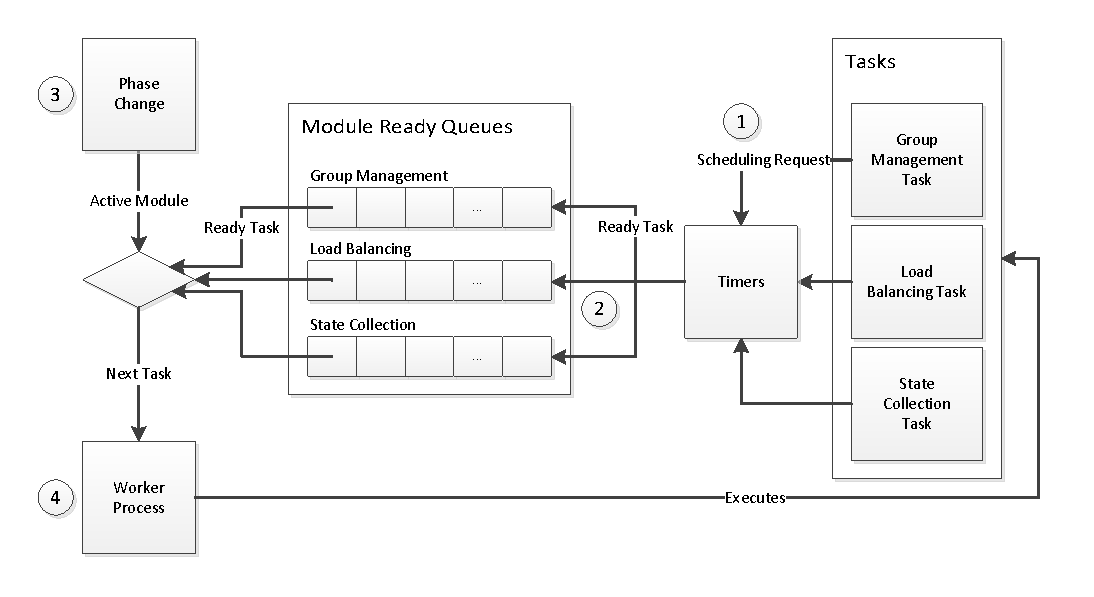
\includegraphics[width=1.0\textwidth]{RealTimeScheduler.pdf}
\captionsetup{singlelinecheck=off}
\caption[Real Time Scheduler]{The realtime scheduler uses a round robin approach to allot execution time to modules. 
\begin{enumerate}
    \item Modules request that a task be executed by specifying a time in the
          future to execute a task. A timer is set to count down to the
          specified moment. Modules may also place tasks immediately into the
          ready queue if the task may be executed immediately.
    \item When the timer expires the task is placed into the ready queue for
          the module that requested the task be executed.
    \item Modules are assigned periods of execution (called phases) which are
          a predetermined length. After the specificed amount of time has
          passed, the module's phase ends and the next module in the schedule's
          tasks begin to execute.
    \item The worker selects the next ready task for the active module from the
          ready queue and executes it. These tasks may also schedule other tasks
          to be run in the future.
\end{enumerate}
}
\label{fig:REALTIMESCHEDULER}
\end{figure}

Modules inform the scheduler of tasks it wishes to perform by either submitting
them to be performed at some point in the future, or informing the scheduler of
a tasks that is ready to be executed immediately.

Tasks that have become ready, either by being inserted as ready, or the time
period that specified when it should be executed after has passed. The prepared
task is inserted into a ready queue for the module that the task has been
scheduled for.

When that modules phase is active, the task is pulled from the ready queue and
executed. When the phase is complete, the scheduler will stop pulling tasks
from the previous modules queue and begin pulling from the next modules queue.

This allows enforcement upper bound message delay. The modules have a specific
amount of processing time allotted. Modules with messages that invoke responses
(or a series of queries and responses) typically are required to be received
within the same phase, using round numbers which enforce that the message was
sent within the same phase.

Modules are designed and allotted time to allow for parameters such as maximum
query-response time (based on the latency between communicating processes). 
This implies that a module which engages in these activities has an
upper-bound in latency before messages are considered lost.

\section{Markov Models}
Understanding how the dynamics of group formation is captured in a Markov Model 
is critical for both assessing its applicability and accuracy in this 
application. First, however, the dynamics of group membership must be 
understood as part of the distributed system.

Consider a set of processes, which are linked by some packet based network 
protocol. In our experiments we provide two protocols, each with different 
delivery characteristics. Under ideal conditions a packet sent by one process 
will always be delivered to its destination. Without a delivery protocol, as 
soon as packets are lost by the communication network, the message that it 
contained is lost forever. Therefore to compensate for the network losing 
packets, a large variety of delivery protocols have been adapted. Each protocol 
has a different set of goals and objectives, depending on the application.

Keeping in mind that a single lost packet does not necessitate the message it 
contained is forever lost, different protocols allow for different levels of 
reliability despite packet loss.

The leader election algorithm is centered around two critical events: checking, 
and elections. The check system is used to detect both failures and the 
availability of nodes for election.

Consider a set of processes which have already formed a group. These processes 
occasionally exchange messages to determine if the other processes have 
crashed. These processes can be classified into two sets: Leaders and Members.

When a leader sends its check messages, the nodes that receive it either 
respond in the positive, indicating that they are also leaders, or in the 
negative indicating that they have already joined a group. This message is sent 
to all known nodes in the system. If a process replies that it is also a 
leader, the original sender will enter and election mode and attempt to combine 
groups with the first process. Nodes that fail to respond are removed from the 
leaders group, if they were members.

The member on the other hand will only direct its check message to the leader 
of its current group. As with the leader's check message, the response can 
either be positive or negative. A yes response indicates that the leader is 
still available and considers the member a part of its group. A no response 
indicates that either the leader has failed and recovered, or it has suspected 
the member process of being unreachable (either due to crash or network issue) 
and has removed them from the group. In this event the member will enter a 
recovery state and reset itself to an initial configuration where it is in a 
group by itself.

On any membership change, either due to recovery, or a suspected failure, the 
list of members for a group is pushed to every member of that group by the 
leader. Members cannot suspect other processes of being crashed, only the 
leader can identify failed group members.

During elections, a highest priority leader (identified by its process id) will 
send invites to the other leaders it has identified. If those leaders accept 
the highest priority leader's invites, they will reply with an accept message 
and forward the invite to their members, if their are any. If the highest 
priority process fails to become the leader the next highest will send invites 
after a specified interval has passed.

Therefore, the membership of the system can be affected in two ways: election 
events which change the size of groups and failure suspicion (via checks) which 
decreases the size of groups. Note that elections can decrease the size of 
groups as well as increase them: If a round of forwarding invites fails by the 
new leader to his original group, the group size could decrease.

When a process is initialized it begins in the "solo" state: it is in a group 
with itself as the only member. As nodes are discovered by checks, the 
processes combine into groups. Groups are not limited by increasing one a time; 
they can increase by combined size of the groups of the leader processes.

The result is similar to a life death process with more complex skips forward 
or backward across the population.

We define a metric to assess the performance of the system under duress, we 
first consider that the distributed can only perform meaningful work when the 
processes can work together to perform physical migration. This means that 
there are two networks that affect the system's ability to do work: the 
physical and the cyber.

Nodes may be separated into distinct partitions. The cyber and physical systems 
can span different nodes 

\chapter{Experimental Design}

Tests were the system were completed by applying network settings and then running the nodes in the prescribed configuration for ten minutes (using the UNIX timeout command). At this point the test was terminated and the group management system appends statistics to an output file. New settings were applied and the next test was begun.

\section{Tools Used, Systems Used}

The application of settings and the initiation of tests was completed using a custom script written in Python. This script used a library, Fabric \cite{FABRIC}, to start runs of the system by the secure shell (SSH). This was run on one of the machine and monitored the I/O of all nodes to ensure everything was behaving correctly.

Our experimental software also provided for ``bussing,'' where a group of edges would
have the same reliability and were iterated together, and ``fixing,'' which allowed for edges that would not change reliability across any of the runs.

All tests were run on four Pentium 4 3GHz machines with 1GB of RAM and Hyper-threading. Tests were run on an ArchLinux install using a real-time kernel, however, the snapshot of the FREEDM software used to run the tests does not feature a real-time scheduler.

The testing software was responsible for initializing instances, allowing them to run and then terminate after a fixed time limit. Additionally it provided an iterative object which generated network settings which were copied to the target machines before each test began.

Each node recorded its own state information, which was appended to a log file at termination of the run. This data was then coupled with the experimental procedure data to create the tables and charts in the results.

For each run of the system, the first 60 seconds of the system were not logged to filter out transients. This leads to a maximum recordable in-group time of nine minutes.
\section{Tests Performed}

Our experiments considered two configurations of the system which can be considered highly characteristic of most other scenarios. The first, a two node configuration was intended to observe a slice of the behavior of the system when two nodes (a leader and a group member) struggle to communicate with one another.

The second configuration was a four node configuration with a transient partition, where the nodes were divided into pairs. Each pair of nodes could reliably communicate with each other, but reliable communication across pairs was not guaranteed. We would vary the reliability of the connection between the pairs and observe the effects on the system.

For both tests, we ran the system using both our sequenced reliable protocol as well as our sequenced unreliable protocol. Additionally, we varied the amount of time between resends for both protocols. A full list of the tests we performed are listed in Table \ref{TableTests}.

In each test, we recorded the number of elections which began, the number that completed successfully, the amount of time spent working on elections, the amount of time spent in a group, and the mean group size. Using these metrics, we hoped to capture a good representation of what kind effects network problems could have on the stability of the groups formed.

\begin{table}[!t]
% increase table row spacing, adjust to taste
\renewcommand{\arraystretch}{1.3}
\caption{Tests Performed}
\label{TableTests}
\centering
% Some packages, such as MDW tools, offer better commands for making tables
% than the plain LaTeX2e tabular which is used here.
\begin{tabular}{c c c c c}
\hline
Test No. & Test Type & Protocol & Resend Time & Window Size \\ \hline \hline
1        & 2 Node    & SRC      & 200ms       & N/A \\ \hline
2        & 2 Node    & SUC      & 200ms       & 8 \\ \hline
3        & 2 Node    & SRC      & 100ms       & N/A \\ \hline
4        & 2 Node    & SUC      & 100ms       & 8 \\ \hline
5        & Transient & SRC      & 200ms       & N/A \\ \hline
6        & Transient & SUC      & 200ms       & 8 \\ \hline
7        & Transient & SRC      & 100ms       & N/A \\ \hline
8       & Transient & SUC      & 100ms       & 8 \\ \hline
\end{tabular}
\end{table}

% RESULTS
%   - Show the unbounded Queue Graph and the mess it makes of LB and GM
%   - Show soft ECVN allows more work to be done, possibly at the cost of accumulating K.
%   - Shwo that HARD ecn allows the best operation -- work gets done and less K is accumlated.

\chapter{Conclusion}

This work presented a new approach for predicting the behavior of a real-time distributed system under omission failure conditions. By using a continuous time Markov chain, a variety of insights can be gathered about the system, including observations such as how long a particular configuration will be stable, and the behavior of the system in the long run.  The Markov results will be used  to make better real time schedules to better react to the network faults we plan on introducing to our test beds. The primary concern are scenarios in which the cyber controller attempts to make physical components which are not connected in the physical network interact, and scenarios where a fault in the cyber network causes the paired events (where two physical controllers change to accomplish some transaction or exchange) to only be partially executed. For example, in the DGI load balancing scheme, a node in a supply state injects a quantum of power into the physical network, but the node in the demand state does not change to accept it. These errors, which are the primary focus of this work could cause instability if a sufficient number of these failed exchanges occur. In \cite{HARINI}, Choudhari et. al. show that failed transactions can create a scenario where the frequency of a power system could become unstable. 

Moving forward, we have identified these areas as targets for improving the research done and creating new contributions.

\section{Time between reconfigurations}

 The rate that the system should reconfigure is a function of the maximum number of failed migrations that the system can handle before becoming unstable, the time it takes to write to the channel and the time it takes process messages. The amount of time in group can also be a consideration for which algorithm to select based on the needed amount of time to perform its work. Group Management can be used as a critical component in a real-time distributed system to manage the number of lost messages and as a consequence, the number of failed migrations in a CPS. It is critical to understand how frequently nodes enter and exit the group based on lost messages and how many migrations fail as a consequence of those messages. This area is deficient because it is strongly coupled to the interactions with the physical component: we must understand how the cyber configuration and physical changes made by that configuration can affect the system, and establish when reconfigurations should occur to keep the system stable. To correct this, we hope to develop a mathematical relationship between the stability of the group, and the physical management functionality of the CPS.

\section{Correctness of an Installed Configuration}

 The work presented in this document is probabilistic: the results of a leader election are random and based only on responses arriving with in a specified period of time. Other factors can affect what configurations can be installed such as trust in the parties in the group, the underlying physical topology, and the reliability of the peers in that group. We hope to develop guarantees on the properties of a configuration that protect the physical topology and the members of the group. These guarantees would also allow processes to better police the configurations they are installed in, in order to protect the system from malicious nodes.

\section{Accuracy of The Model}

We recognize that the model presented thus far does not have ideal accuracy. We expect to be able to further refine the model and the algorithms and formulas for generating the model. There are some features of the behavior of the DGI which are not completely encapsulated in the model. Additionally, the way models are specified can be generalized to support more systems of similar design. As part of this work however, we must remember modeling distributed systems is extremely difficult and while the increase in accuracy is desirable it is not a critical goal.

\section{Scope of the Model}

The models presented in this work focus only on the leader election component of a dynamically configured CPS. Additional work would incorporate additional components of the DGI system into the models for a more complete picture of the behavior of the system during failures. We will consider the correctness of the incorporated algorithms, how omission failures can violate that correctness, and what restrictions we can place on the configuration and operation of DGIs in order to protect the entire system during failures. To do this, we will expand the analysis performed here to incorporate algorithms such as state collection and load balancing and define metrics to quantify their behavior during omission failures. This thrust will pair with the correctness and time between reconfigurations: different algorithms will have different amounts of failure that can be allowed before reconfiguration is necessary.

\section{Deliverables}

Therefore, moving forward, we will expand the models we have presented here to include more of the properties of the complete CPS. This model will allow us to better understand what effects the group behavior has on the CPS. Using this, we can establish invariants which allow us to ensure the correctness of a CPS by providing assertions which will not be broken during execution. Creating these invariants will allow us to improve the development of CPSs, especially in their dynamic configuration, which is an area with limited development. These invariants also allow us to create an assertion of correctness which can be validated, during runtime, to ensure the system maintains its stability. We will continue to create and validate models of the CPS against simulations and actual hardware. As we do so we will construct invariants that describe the correct behavior of the groups to ensure safe operation. In addition to the existing conference paper \cite{CRITIS2012}, we have prepared a journal paper with the new work in this document. 
%\lipsum[1-20]% to test page spacing
%\end{ThesisBackMatter}
\end{ThesisBody}

\begin{ThesisAppendix}{three}
%\chapter{Characteristic Length Scales}
\label{sec:lengths}
%This table lists lengths used in the dissertation.

\captionsetup[table]{list=no}
%\begin{center}
\begin{table} % for label and caption purposes
%\begin{tabular}{|l|l|l|} % table runs off page
%\begin{tabular}{|l|l|p{7cm}|} % center column too large
\caption{Length scales used in this dissertation}
\begin{tabular}{|l|p{4cm}|p{8.5cm}|}
%\begin{tabular*}{0.75\textwidth}{|l|l|l|}{@{\extracolsep{\fill}} | c | c | c | }
\hline Symbol & Name & Description \\ \hline
$\lambda$ & wavelength & Wavelength of incident light \\ 
$L$ &  system length & Length of waveguide along direction of propagation ($z$-axis) \\ 
$W$ & system width & Dimension of waveguide perpendicular to direction of propagation ($y$-axis) \\
$L_{\phi}$ & phase coherence length & Length over which phase remains coherent. Equivalent to $L_{inelastic}$\cite{1988_Stone,1986_Imry}. Applicable only to electron transport. \\
$L_D$ & path length & How far a particle (i.e. ray optics) travels in the media in ballistic and diffusive regimes \\
$\ell_{scat}$ & scattering length & Average distance between scattering events. Often referred to as $\ell_{mfp}$ (mean free path) or the inelastic length\cite{1984_John_prl}, or extinction length\cite{1999_van_Tiggelen}. \\ 
$\ell_{tmfp}$ & transport mean free path & Average distance over which phase and direction are randomized.  $\ell_{tmfp} = \frac{\ell_{scat}}{1-\langle cos\ \theta \rangle}$. Sometimes referred to as elastic mfp\cite{1991_John}. % page 34, col 2
Measured with respect to $L$. \\ 
$\xi$ & localization length & Probability of diffusive path forming loop is 1. $\xi~=~N~\ell_{tmfp}$. Measured with respect to $L$. \\ 
$\ell_{a,g}$ & ballistic absorption/gain length & Average distance over which intensity decreases by two/increases by two. \\
$\xi_{a,g}$ & absorption/gain length & How far, on average, a particle travels in the diffusive regime before being absorbed (or doubled), measured with respect to path length $L_D$ in the diffusive regime \\ 
$z_p$ & penetration depth & Applies to diffusive regime only. $z_p \approx \ell_{tmfp}$ \\ 
\hline
\end{tabular}

\ \\ 

\label{tabl:lengths}
\end{table}
%\end{center}
All length scales (except $\lambda$) are normalized by wavelength. % lengths can be converted to equivalent times by $\ell = c t$
%\captionsetup[table]{list=yes} % referenced in introduction
%\chapter{Transmission Derivation}

This is an expanded version of the analysis performed for Fig.~\ref{fig:energydistrib}

\begin{equation}
T = T(\omega, x_o) = \frac{(\exp(-\frac{L}{\xi}))^2}{ 
(\omega-\omega _o)^2 + (\exp(-\frac{L}{\xi})\frac{1}{2}\exp(\frac{\mid L-2 x_o \mid}{\xi}))^2 }
\label{fig:appendixtransmission}
\end{equation}
Where we have appoximated cosh() as $\frac{1}{2}\exp()$. 

From the behavior of transmission in media with defects and centers of localizaiton, we see two cases when on a resonant frequency:  either the defect is in the first half of the sample.%, (\ref{fig:cononicaldefectpositions}, plot 1).

\begin{equation}
{\cal E}(x) = \left\{ 
\begin{array}{l l}
  A \exp\left(\frac{2 (x-x_o)}{\xi}\right) & \quad 0 < x < x_o \\
  B \exp\left(-\frac{2 (x-x_o)}{\xi}\right) & \quad x_o < x < L\\
\end{array} \right.
\label{fig:left}
\end{equation}

or it is in the second half of the sample.%, (\ref{fig:cononicaldefectpositions}, plot 2).
\begin{equation}
{\cal E}(x) = \left\{ 
\begin{array}{l l}
 A \exp\left(-\frac{2 x}{\xi}\right) & \quad 0 < x < L-2 x_o \\
 B \exp\left(\frac{2 (x-x_o)}{\xi}\right) & \quad L-2 x_o < x < x_o \\
 C \exp\left(-\frac{2 (x-x_o)}{\xi}\right) & \quad x_o < x < L \\
\end{array} \right.
\label{fig:right}
\end{equation}

With either case, we see three distinct regions when the frequency is not on resonance but prior to the pure exponential decay regimes. %(\ref{fig:cononicaldefectpositions}, plot 3):
\begin{equation}
{\cal E}(x) = \left\{ 
\begin{array}{l l}
y_1 = A \exp\left(-\frac{2 x}{\xi}\right)   & \quad 0 < x < x_1  \\
y_2 = B \exp\left(\frac{2 (x-x_o)}{\xi}\right) & \quad x_1 < x < x_o  \\
y_3 = C \exp\left(-\frac{2 (x-x_o)}{\xi}\right) & \quad  x_o < x < L \\
\end{array} \right.
\label{fig:startingequations}
\end{equation}
Where $x_1$ is the turning point.

\begin{comment}
%% pictures were removed, causes a problem during compile (?)
\begin{figure}
\vskip -0.5cm
\centerline{
\scalebox{0.5}{\includegraphics{pictures/transmission_derivation_14_LR}}
\scalebox{0.5}{\includegraphics{pictures/transmission_derivation_34_LR}}
\scalebox{0.5}{\includegraphics{pictures/transmission_derivation_off_res_LR}}
}
\vskip -0.5cm
\caption{Log of energy versus position sketches for a center of localization in the first half (left), Eq.~\ref{fig:left}; and second half (center), Eq.~\ref{fig:right}. The turning point in the center plot is $L-2 x_o$. The right sketch is off-resonance but prior to pure exponential decay, which applies to any center of localization position, as described by Eq.~\ref{fig:startingequations}. The turning point in the right plot from the initial exponential decay to growth varies depending how far off resonance one is. We call this $x_1$}
\label{fig:cononicaldefectpositions}
\end{figure}
\end{comment}

From the off-resonance Eq.~\ref{fig:startingequations}, we apply boundry conditions to determine the coefficients in passive systems. We take gain into account and make corrections later.

At $x=0$ then $y_1=4$, giving $A=4$. Thus
\begin{equation}
\boxed{y_1 = 4 \exp\left(-\frac{2 x}{\xi}\right)}   \quad \quad \quad 0 < x < L-2 x_o 
\end{equation}

At $x=L$, $y_3=T$. Solve for C,
\begin{equation}
C=T \exp\left(\frac{2(L-x_o)}{\xi}\right)
\end{equation}
plug back in,
\begin{equation}
y_3 = T \exp\left(\frac{2(L-x_o)}{\xi}) \exp(-\frac{2 (x-x_o)}{\xi}\right)  \quad \quad \quad  x_o < x < L
\end{equation}
simplify to get
\begin{equation}
\boxed{y_3 = T \exp\left(-\frac{2(x-L)}{\xi}\right)}  \quad \quad \quad  x_o < x < L
\end{equation}
at $x_o$, $y_2 = y_3$
\begin{equation}
B \exp\left(\frac{2 (x_o-x_o)}{\xi}\right) = B = T \exp\left(-\frac{2(x_o-L)}{\xi}\right)
\end{equation}
plug in to $y_2$
\begin{equation}
y_2 = T \exp\left(-\frac{2(x_o-L)}{\xi}\right) \exp\left(\frac{2 (x-x_o)}{\xi}\right) \quad \quad \quad L-2 x_o < x < x_o 
\end{equation}
simplify to get
\begin{equation}
\boxed{y_2 = T \exp\left(\frac{2(x+L-2 x_o)}{\xi}\right)} \quad \quad \quad L-2 x_o < x < x_o 
\end{equation}

The turning point $x_1$ varies as a function of frequency. Boundry conditions on $x_1$ are that it should remain less than $x_o$ and that it be non-negative. To solve for $x_1$, see where $y_1=y_2$
\begin{equation}
4 \exp\left(-\frac{2 x_1}{\xi}\right) = T \exp\left(\frac{2(x_1+L-2 x_o)}{\xi}\right)
\end{equation}

\begin{equation}
\boxed{x_1(\omega) = -\frac{\xi}{4} \log(\frac{1}{4} T) - \frac{1}{2}L + x_o}
\end{equation}

Knowing $y_1,y_2$, and $y_3$ we can integrate to find the energy ${\cal E}$:
\begin{equation}
\begin{gathered}
{\cal E}(x,\omega) = \int _0 ^{x_1} 4 \exp\left(-\frac{2 x}{\xi}\right) dx +
    \int _{x_1} ^{x_o} T \exp\left(\frac{2(x+L-2 x_o)}{\xi}\right) dx + \\
    \int _{x_o} ^{L} T \exp\left(-\frac{2(x-L)}{\xi}\right)
\label{fig:Eintegral}
\end{gathered}
\end{equation}

Solve, reduce to get the energy as a function of x, frequency, and transmission:
\begin{equation}
\begin{gathered}
{\cal E}(x,\omega) = \frac{\xi}{2} \left( T \left( \exp\left(\frac{2(L-x_o)}{\xi}\right) - \exp\left(\frac{2(L-2 x_o+x_1)}{\xi}\right)+\right. \right.\\
\left.\left.\exp\left(\frac{2(L-x_o))}{\xi}\right) -1 \right) + 4 \left(1-\exp\left(-\frac{2 x_1}{\xi}\right)\right) \right)
\label{fig:appendixenergy}
\end{gathered}
\end{equation}

 % expansion of math in T/E paper
%%\chapter{Derivation of Transfer Matrices for Electric Field Propagation in Planar Quasi-1D Waveguide From Maxwell's Equations}
\chapter{Transfer Matrices for Electric Field Propagation}
\label{sec:appendix_derivation_transfer_matrices_quasi1d}

In the following derivation, the transfer matrix method\cite{1981_MacKinnon_scaling}\cite{1992_Pendry}\cite{2003_Kettemann} is developed from Maxwell's equations\cite{1999_Jackson}. Before starting, the assumptions necessary for the derivation are enumerated. 
\begin{itemize}
\item No leakage of electric field at edge ($y=0$, $y=W$) of waveguide (i.e. metallic boundaries). Gives boundary conditions of zero field at edges. Incident and output edges are open (no restrictions).
\item $\delta$-function scattering potentials, later reduced to a finite sum of Fourier components. Use of this scattering potential has generalized results
%   \item non-physical
%   \item infinite number of closed channels
\item No inelastic scattering: no energy loss due to scattering when passive, and phase remains coherent [scatterers only affect amplitude].
\item No noise (spontaneous emission). We are interested primarily in the AL/diffusion phenomenon. Also, experimentally noise can be suppressed. % CITE
%The transmission with gain will be slightly different compared to real output.
\item The gain mechanism is purely mathematical: no atomic level modeling is included. This is part of being mesoscopic regime: independent of atomic-based scattering mechanisms.
\item No input beam properties are assumed (can be plane wave, but that is not necessary).%, other than the capability to be selectively incident on a specific channel.
%\item By choosing planar quasi-1D geometry (and thus scalar waves), we implicitly assume that polarization will not significantly alter transport phenomena. Although planar geometry may be experimentally realizable, it is not as popular as 3D quasi-1D
\end{itemize}

%\section{From Maxwell equations to wave equation}
%Starting with Maxwell's equations, the wave equation for electromagnetic waves is derived to demonstrate that only a single polarization is being studied. Ampere's Law (with current $\vec{J}=0$ and $D=\epsilon_0 E$)\cite{1999_Jackson}, %Eq. I.1b, page 2
%\begin{equation}
%\vec{\nabla} \times \vec{{\cal H}} = \epsilon_0 \frac{\partial\vec{E}}{\partial t}
%\label{eq:amperes_law}
%\end{equation}
%Faraday's Law \cite{1999_Jackson}, %Eq. I.1a, page 2]
%\begin{equation}
%\vec{\nabla} \times \vec{E} = -\mu_0 \frac{\partial\vec{{\cal H}}}{\partial t}
%\label{eq:faradays_law}
%\end{equation}
%Taking the temporal derivative of Eq.~\ref{eq:amperes_law}
%\begin{equation}
%\vec{\nabla} \times \frac{\partial\vec{{\cal H}}}{\partial t} = \epsilon_0 \frac{\partial^2\vec{E}}{\partial t^2}
%\label{eq:temporal_derivative_of_amperes_law}
%\end{equation}
%Taking the curl of Eq.~\ref{eq:faradays_law}
%\begin{equation}
% \vec{\nabla} \times \vec{\nabla} \times \vec{E} = -\mu_0 \left(\vec{\nabla} \times \frac{\partial\vec{{\cal H}}}{\partial t} \right)
%\label{eq:curl_of_faradays_law}
%\end{equation}
%Substitute Eq.~\ref{eq:temporal_derivative_of_amperes_law} into Eq.~\ref{eq:curl_of_faradays_law}
%\begin{equation}
%  \vec{\nabla} \times \vec{\nabla} \times \vec{E} = -\mu_0 \epsilon_0 \frac{\partial^2\vec{E}}{\partial t^2}
%\end{equation}
%Vector identity: $\vec{\nabla} \times \vec{\nabla} \times \vec{E} = \vec{\nabla} (\vec{\nabla}\cdot \vec{E})-\nabla^2 \vec{E}$. Since we assume no source, we have the wave equation

The wave equation is derived from Maxwell's equations (not show). In the following, only $s$-polarized waves (for transverse-magnetic (TM) waves) are assumed incident: electric field oscillates perpendicular to the plane of the 2D waveguide.
%``For EM waves propagating in the $z,y$ plane, the $s$ ($E$ field parallel to the $x$ axis) and $p$ ($E$ field perpendicular to the $x$ axis) polarized waves can be described by two decoupled wave equations.'' 
\cite{1996_soukoulis_dis2d}
\begin{equation}
\nabla^2 E = \frac{1}{c^2} \frac{\partial^2\vec{E}}{\partial t^2}
\label{eq:general_wave_equ}
\end{equation}
where $\mu_0 \epsilon_0 = \frac{1}{c^2}$. 
%[See 1996 Soukoulis et al PRB v53 n13 pg 8340, section II] 
% Eq.~\ref{eq:general_wave_equ} ``is identical with the scalar wave equation.'' The $p$-polarized wave equation involves ${\cal H}$.

\section{Time Independent Wave Equation}
Assuming electric field variables are separable,
\begin{equation}
E(\vec{r},t) = E(\vec{r}) e^{i\omega t}
\label{eq:separation_of_variables_E_field}
\end{equation}
the field is simplified by also assuming monochromatic and continuous wave (CW). Substituting  Eq.~\ref{eq:separation_of_variables_E_field} into the right side of Eq.~\ref{eq:general_wave_equ}, time dependence can be canceled. 
\begin{equation}
\nabla^2 E(\vec{r}) = - \frac{\omega^2}{c^2} E(\vec{r})
\label{eq:wave_equation_electric_field}
\end{equation}
where $\frac{\omega}{c}=k$. Although the following results will appear to be ``time independent,'' the time dependence can be reintroduced by multiplying both sides by $e^{i\omega t}$. Effectively the same as assuming $t=0$. 


\section{Separation of Variables}
Convert from general $\vec{r}$ to two-dimensional Cartesian coordinates (since the transfer matrices for a planar quasi-1D waveguide are desired): $\vec{r} = z \hat{i}+y\hat{j}$. Let $W \equiv$ width and $L \equiv$ length of waveguide.
%\begin{equation}
%\vec{r} = z \hat{i}+y\hat{j}
%\end{equation}
%and the Laplacian is
%\begin{equation}
%\nabla^2 = \frac{\partial^2}{\partial z^2} + \frac{\partial^2}{\partial y^2}
%\label{eq:laplacian_cartesian}
%\end{equation}

%unjustified claim
The $z$ and $y$ components of the field are independent, the separation of variables applies spatially.
\begin{equation}
E(\vec{r}) = E(z,y) = \sum^\infty_{n=1} E_n(z) \chi_n(y)
\label{eq:spacialseparation}
\end{equation}
where the sum is over all channels. For $\delta$-function scatterers, there can be an infinite number of closed channels.

Now the wave equation (Eq.~\ref{eq:wave_equation_electric_field}) is 
\begin{equation}
\nabla^2 E(z,y) = - \frac{\omega^2}{c^2} E(z,y)
\label{eq:wave_equation_electric_field_cartesian}
\end{equation}
Apply Laplacian %(Eq.~\ref{eq:laplacian_cartesian}) 
and separation (Eq.~\ref{eq:spacialseparation})
\begin{equation}
\sum^\infty_{n=1} \left[ \frac{\partial^2E_n(z)}{\partial z^2} \chi_n(y) + E_n(z) \frac{\partial^2 \chi_n(y)}{\partial y^2} \right] = \\
- \frac{\omega^2}{c^2} \sum^\infty_{n=1} E_n(z) \chi_n(y)
\label{eq:summation_variable_separation_cartesian}
\end{equation}

\section{Perpendicular Component Solution}
The solution to the differential equation perpendicular to the direction of propagation is found from the auxiliary equation for each channel
\begin{equation}
\left(\frac{\partial^2}{\partial y^2} + k_{\bot n}^2 \right) \chi_n(y) = 0
\end{equation}
Boundary conditions for metallic waveguide: Electric field $E$ is zero at the boundaries, $\chi_n(0) = \chi_n(W) = 0$.
%\begin{equation}
%\chi_n(0) = \chi_n(W) = 0
%\end{equation}
The normalized solution is the familiar
\begin{equation}
\chi_n(y) = \sqrt{\frac{2}{W}} \sin (k_{\bot n} y)
\end{equation}
where 
%\begin{equation}
$k_{\bot n} \equiv \frac{n \pi}{W}$. 
%\label{eq:k_perpendicular}
%\end{equation}
As a check of normalization, for $m=n$
\begin{equation}
\int^W_0 \chi_n^2(y) dy = \frac{2}{W} \int^W_0 \sin^2 (k_{\bot n} y) = \frac{2}{W} \frac{1}{2} W = 1
\end{equation}
and if $m \neq n$, solutions are orthogonal
\begin{equation}
\int^W_0 \chi_n(y)\chi_m(y) dy = 0
\end{equation}
Thus, for general $n$ and $m$,
\begin{equation}
\int^W_0 \chi_n(y)\chi_m(y) dy = \delta_{n,m}
\label{eq:convert_to_kronecker}
\end{equation}

\section{Parallel Component Solution}
For the solution parallel to the direction of propagation of Eq.~\ref{eq:wave_equation_electric_field_cartesian}, the $z$-component starts with
\begin{equation}
\frac{\partial^2 E_n(z)}{\partial z^2} - k_{\bot n}^2 E_n(z) = - \frac{\omega^2}{c^2} E_n(z)
\end{equation}
Re-arrange and introduce a new variable
\begin{equation}
\frac{\partial^2 E_n(z)}{\partial z^2} + k_{\parallel n}^2 E_n(z) = 0
\label{eq:zcomponentdiffequ}
\end{equation}
where
\begin{equation}
k_{\parallel n}^2 \equiv \frac{\omega^2}{c^2} - k_{\bot n}^2
\label{eq:k_parallel}
\end{equation}
Note: $k_{\parallel n}^2$ can be positive (corresponding to open channels) or negative (closed channels). If negative, then $k_{\parallel n}$ is imaginary, denoted $k_{\parallel n} = i \kappa_{\parallel n}$ for $n > N_{open}$. Open channels propagate forward, with velocity decreasing as channel index increases. Closed channels decrease in amplitude exponentially.

%The summation in Eq.~\ref{eq:summation_variable_separation_cartesian} can be split into open and closed channels
%\begin{equation}
%\sum_{n=1}^\infty = \sum_{n=1}^{N_o} + \sum_{n=N_{o}+1}^\infty	
%\end{equation}

%\begin{tabular}{cc}
%$ n \leq N_o $ \quad \quad \quad & $ k_{\parallel n}^2 = \frac{\omega^2}{c^2} - \left(\frac{n \pi}{W}\right)^2 > 0 $ \\
%$ n > N_o $ \quad \quad \quad & $ k_{\parallel n}^2 < 0 $ \\
%\end{tabular}

Separate electric field components into left(-) and right (+) traveling plane waves (two solutions to the second order differential equation)
\begin{equation}
\begin{gathered}
\text{Open: \ }  E_n(z) = E_n^+ \exp(i k_{\parallel n} z) + E_n^- \exp(-i k_{\parallel n} z) \\
\text{Closed: \ }   E_n(z) = E_n^+ \exp(-\kappa_{\parallel n} z) + E_n^- \exp(\kappa_{\parallel n} z) 
\end{gathered}
\label{eq:Eleftandrightpropagating}
\end{equation}
where $i \kappa \equiv k$

\section{Waveguide With Scatterers}
Up to this point, an empty waveguide has been considered. For scattering, replace $\frac{\omega^2}{c^2}$ of the wave equation \ref{eq:wave_equation_electric_field_cartesian} with a spacial Sellmeier equation
\begin{equation}
\frac{\omega^2}{c^2} (1 + \alpha \delta(z-z_0,y-y_0))
\label{eq:scatterer}
\end{equation}
where $\delta(z-z_0,y-y_0) \equiv \delta(z-z_0) \delta(y-y_0)$ is the scattering potential and $\alpha$ is the scattering strength. $\alpha$ can be complex; then the real part is the strength and the imaginary component is gain or absorption.

%Note: this new term changes Eqs.~\ref{eq:amperes_law},\ref{eq:general_wave_equ}, and \ref{eq:wave_equation_electric_field} by introducing a non-unity refractive index.

To determine transport of light past a scattering potential, apply continuity of electric field $E$ and its derivative. The following carries out matching component-wise derivative.

Assuming the scattering potential is located at cross-section $z$ (inside the waveguide $0<z<L$), and the electric field just before or after the scatterer (at $z \pm \Delta$) is a sum of independent channel components.
\begin{equation}
E(z \pm \Delta, y) = \sum_{n=1}^\infty E_n(z \pm \Delta) \chi_n(y)
\end{equation}
Applying Eq.~\ref{eq:scatterer} to Eq.~\ref{eq:zcomponentdiffequ}, the wave equation becomes
\begin{equation}
\sum_{n=1}^\infty \left( E_n^{\prime\prime} \chi_n + k_{\parallel n}^2 E_n \chi_n + \alpha \frac{\omega^2}{c^2} \delta(z-z_0,y-y_0) E_n \chi_n \right) = 0
\label{eq:doubleprimeEz}
\end{equation}

Multiply Eq.~\ref{eq:doubleprimeEz} by $ \chi_m $ and $ \int_0^W dy $. By applying Eq.~\ref{eq:convert_to_kronecker} and letting $A_{m,n}(y_0)=\chi_m(y_0) \chi_n(y_0)$, 
\begin{equation}
\sum_{n=1}^\infty \left( E_n^{\prime\prime} \delta_{nm} + k_{\parallel n}^2 E_n \delta_{nm} + \alpha \frac{\omega^2}{c^2} E_n \delta(z_0) A_{nm}(y_0)  \right) = 0 
\end{equation}
Apply the summation over $n$, which eliminates the Kronecker deltas.
\begin{equation}
 E_m^{\prime\prime} + k_{\parallel m}^2 E_m + \alpha \frac{\omega^2}{c^2} E_n \delta(z-z_0) \sum_{n=1}^\infty A_{nm}(y_0) = 0
\end{equation}
Integrate over $z$ from $(z-\Delta)$ to $(z+\Delta)$ and let $\Delta\rightarrow0$.
\begin{equation}
\begin{gathered}
\int_{z_0-\Delta}^{z_0+\Delta} E_m^{\prime\prime}(z) dz + k_{\parallel m} ^2 \int_{z_0-\Delta}^{z_0+\Delta} 
E_m(z) dz +\\ \alpha \frac{\omega^2}{c^2} \sum_{n=1}^\infty A_{n,m}(y_0) \int_{z_0-\Delta}^{z_0+\Delta} \delta(z_0) E_n dz = 0
\end{gathered}
\end{equation}

To do the second term integration, assume that for small $\Delta$, $E(z) \approx E(z_0)$.  
\begin{equation}
E_m^{\prime}(z_0 + \Delta) - E_m^{\prime}(z_0 - \Delta) + k_{\parallel m}^2 E_m(z_0) 2 \Delta + \alpha \frac{\omega^2}{c^2} \sum_{n=1}^\infty A_{n,m}(y_0) E_n(z_0) = 0
\end{equation}

Since $\Delta \rightarrow 0$, then $2 \Delta$ is really small, so that term is dropped.

To conclude, for a given channel $m$, electric field and the field derivative on both sides of the scatterer must match
\begin{equation}
\begin{gathered}
%\boxed{
E_m(z_0+\Delta) = E_m(z_0-\Delta) \\
%}
%\\
%\boxed{
E_m^{\prime}(z_0+\Delta) = E_m^{\prime}(z_0-\Delta) - \alpha \frac{\omega^2}{c^2} \sum_{n=1}^\infty A_{n,m}(y_0) E_n(z_0)
%}
\end{gathered}
\end{equation}

Note that the $\delta$ function scatterer has been eliminated, and $A_{n,m}$ can form an array (the ``scattering matrix'').

\begin{equation}
\begin{gathered}
\left( \begin{array}{cc}
\hat{I} & 0 \\
-\alpha \frac{\omega^2}{c^2}A_{mn}(y_0) & \hat{I} \\
\end{array} \right)
\left( \begin{array}{c}
E_{1..N_{max}}(z_0-\Delta) \\
\frac{1}{\kappa_{\parallel 1..N_{max}}} E_{1..N_{max}}^{\prime}(z_0-\Delta) 
\end{array} \right)
=\\
\left( \begin{array}{c}
E_{1..N_{max}}(z_0+\Delta) \\
\frac{1}{\kappa_{\parallel 1..N_{max}}} E_{1..N_{max}}^{\prime}(z_0+\Delta) 
\end{array} \right)
\end{gathered}
\end{equation}
Due to the form of the matrix, the determinant is always unity (only the diagonal contributes non-zero terms) regardless of the elements in the lower left quadrant. Elements of the lower left quadrant are
\begin{equation}
 -\alpha \frac{\omega^2}{c^2} \frac{2}{W} \sin(k_{\perp m} y_0) \sin(k_{\perp n} y_0)
\end{equation}
Note that the scattering matrix is real unless $\alpha$ or $\omega$ are complex.

\section{Free Space Propagation of Open Channels}
For open channels ($n \leq N_o$), field $E_n$ and derivative of field $ \frac{1}{k_{\parallel n}}E_n^{\prime}$ are more convenient basis than ``left traveling'' $E_n^-(z)$ and ``right traveling'' $E_n^+(z)$. First, the connection between the two basis is found. Starting from Eq.~\ref{eq:Eleftandrightpropagating}, electric field $E(z)$ is the solution to a second order differential equation, so it has two solutions.
\begin{equation}
\begin{gathered}
E_n(z) = E_n^+ \exp(i k_{\parallel n} z) + E_n^- \exp(-i k_{\parallel n} z) \\
E_n^{\prime}(z) = i k_{\parallel n} E_n^+ \exp(i k_{\parallel n} z) - i k_{\parallel n}E_n^- \exp(-i k_{\parallel n} z)
\label{eq:Eleftandrightpropagating_again}
\end{gathered}
\end{equation}
Solving for left- and right-traveling wave components,
\begin{equation}
\begin{gathered}
E_n^+(z) = \frac{1}{2} \left( E_n(z)+\frac{1}{i} \frac{1}{k_{\parallel n}} E_n^{\prime}(z) \right) \exp(-i k_{\parallel n} z) \\ 
E_n^-(z) = \frac{1}{2} \left( E_n(z)-\frac{1}{i} \frac{1}{k_{\parallel n}} E_n^{\prime}(z) \right) \exp(i k_{\parallel n} z) 
\label{eq:Eleftright}
\end{gathered}
\end{equation}

To preemptively clear up notation confusion, in previous steps $\Delta$ was used to denote a small distance away from the scatterer. Here $\Delta z$ will be used to signify a not infinitesimal displacement in position along the $z$ axis. The field and derivative of field is translated over distance $\Delta z$ from the original position $z$. First, substitute the shift into Eq.~\ref{eq:Eleftandrightpropagating_again}
\begin{equation}
E_n(z+\Delta z) = E_n^+ \exp(i k_{\parallel n} (z+\Delta z)) + E_n^- \exp(-i k_{\parallel n} (z+\Delta z)) 
\end{equation}
Then substitute Eq.~\ref{eq:Eleftright}
\begin{equation}
\begin{gathered}
E_n(z+\Delta z) = \frac{1}{2} \left( E_n(z) + \frac{1}{i} \frac{1}{k_{\parallel n}} E_n^{\prime}(z) \right) \exp(i k_{\parallel n} z) + \\
\frac{1}{2} \left( E_n(z) - \frac{1}{i} \frac{1}{k_{\parallel n}} E_n^{\prime}(z) \right) \exp(-i k_{\parallel n} z) 
\end{gathered}
\end{equation}
Reducing leaves how to shift an electric field over distance $\Delta z$.
\begin{equation}
%\boxed{
E_n(z+\Delta z) =E_n(z) \cos(k_{\parallel n} \Delta z) + \frac{1}{k_{\parallel n}} E_n^{\prime} \sin(k_{\parallel n} \Delta z) 
%}
\label{eq:open_channel_field_transfer}
\end{equation}
Similarly,
\begin{equation}
\frac{1}{k_{\parallel n}} E_n^{\prime}(z+\Delta z) = i E_n^+ \exp(i k_{\parallel n} (z+\Delta z)) -i E_n^- \exp(-i k_{\parallel n} (z+\Delta z))
\end{equation}
Then substitute Eq.~\ref{eq:Eleftright}
\begin{equation}
\begin{gathered}
\frac{1}{k_{\parallel n}} E_n^{\prime}(z+\Delta z) =
\frac{i}{2} \left( E_n(z) + \frac{1}{i} \frac{1}{k_{\parallel n}} E_n^{\prime}(z) \right) \exp(i k_{\parallel n} z) -\\
\frac{i}{2} \left( E_n(z) - \frac{1}{i} \frac{1}{k_{\parallel n}} E_n^{\prime}(z) \right) \exp(-i k_{\parallel n} z) 
\end{gathered}
\end{equation}

\begin{equation}
%\boxed{
\frac{1}{k_{\parallel n}} E^{\prime}(z+\Delta z)=- E_n(z) \sin(k_{\parallel n} \Delta z) + \frac{1}{k_{\parallel n}} E_n^{\prime} \cos(k_{\parallel n} \Delta z) 
%}
\label{eq:open_channel_deriv_transfer}
\end{equation}

\section{Free-space Propagation of Closed Channels}
For closed channels ($n > N_o$), change of $i$ results in hyperbolic trig functions.
\begin{equation}
\begin{gathered}
E_n(z) = E_n^+ \exp(-\kappa_{\parallel n} z) + E_n^- \exp(\kappa_{\parallel n} z) \\
E_n^{\prime}(z) = -\kappa_{\parallel n} E_n^+ \exp(-\kappa_{\parallel n} z) + \kappa_{\parallel n}E_n^- \exp(\kappa_{\parallel n} z)
\end{gathered}
\end{equation}
Recalling that $k_{\parallel n} = i \kappa_{\parallel n}$, then
\begin{equation}
\begin{gathered}
E_n^+(z) = \frac{1}{2} \left( E_n(z)- \frac{1}{\kappa_{\parallel n}} E_n^{\prime}(z) \right) \exp(\kappa_{\parallel n} z) \\ 
E_n^-(z) = \frac{1}{2} \left( E_n(z)+ \frac{1}{\kappa_{\parallel n}} E_n^{\prime}(z) \right) \exp(-\kappa_{\parallel n} z) 
\end{gathered}
\end{equation}

Shifting the field by $\Delta z$
%\begin{equation}
%E_n(z+\Delta z) = E_n^+ \exp(-\kappa_{\parallel n}(z+\Delta z)) + E_n^- \exp(\kappa_{\parallel n}(z+\Delta z))
%\end{equation}
%\begin{equation}
%E_n(z+\Delta z) = \frac{1}{2} \left( E_n(z)- \frac{1}{\kappa_{\parallel n}} E_n^{\prime}(z) \right) \exp(-\kappa_{\parallel n} z) +  
%\frac{1}{2} \left( E_n(z)+ \frac{1}{\kappa_{\parallel n}} E_n^{\prime}(z) \right) \exp(\kappa_{\parallel n} z) 
%\end{equation}
\begin{equation}
%\boxed{
E_n(z+\Delta z) = E_n(z) \cosh(\kappa_{\parallel n}\Delta z) + \frac{1}{\kappa_{\parallel n}} E_n^{\prime}(z) \sinh(\kappa_{\parallel n}\Delta z)
%}
\end{equation}
and
%\begin{equation}
%\frac{1}{\kappa_{\parallel n}}E_n^{\prime}(z+\Delta z) = -E_n^+ \exp(-\kappa_{\parallel n}(z+\Delta z)) + E_n^- \exp(\kappa_{\parallel n}(z+\Delta z)) 
%\end{equation}
%\begin{equation}
%\begin{gathered}
%\frac{1}{\kappa_{\parallel n}}E_n^{\prime}(z+\Delta z) =-\frac{1}{2} \left( E_n(z)- \frac{1}{\kappa_{\parallel n}} E_n^{\prime}(z) \right) \exp(-\kappa_{\parallel n} z) + \\
%\frac{1}{2} \left( E_n(z)+ \frac{1}{\kappa_{\parallel n}} E_n^{\prime}(z) \right) \exp(\kappa_{\parallel n} z) 
%\end{gathered}
%\end{equation}
\begin{equation}
%\boxed{
\frac{1}{\kappa_{\parallel n}}E_n^{\prime}(z+\Delta z) =E_n(z) \sinh(\kappa_{\parallel n}\Delta z) + \frac{1}{\kappa_{\parallel n}} E_n^{\prime}(z) \cosh(\kappa_{\parallel n}\Delta z)
%}
\end{equation}

To summarize,
\begin{equation}
\begin{gathered}
E_n(z+\Delta z) = E_n(z) \cosh(\kappa_{\parallel n}\Delta z) + \frac{1}{\kappa_{\parallel n}} E_n^{\prime}(z) \sinh(\kappa_{\parallel n}\Delta z) \\
\frac{1}{\kappa_{\parallel n}}E_n^{\prime}(z+\Delta z) =E_n(z) \sinh(\kappa_{\parallel n}\Delta z) + \frac{1}{\kappa_{\parallel n}} E_n^{\prime}(z) \cosh(\kappa_{\parallel n}\Delta z)
\label{eq:closed_channel_transfer}
\end{gathered}
\end{equation}

From Eq.~\ref{eq:open_channel_field_transfer}, \ref{eq:open_channel_deriv_transfer}, and \ref{eq:closed_channel_transfer} the ``free space propagation matrix'' can be constructed. The array would be of rank $2 n_{max}$ ($n_{max}=N_o+N_c$). The determinant of this matrix is alway unity (regardless of argument) because terms can be factored into $\sin^2x +\cos^2=1$ for each channel. Thus, for both free and scattering matrices, the determinant is unity regardless of free space separation $\Delta z$ or real (passive) and complex (active media) dielectric values.

\begin{comment}
\begin{equation}
\left( \begin{array}{cccccccc}
\cos(k_{\parallel 1}\Delta z)   & 0 & 0 & 0 & \sin(k_{\parallel 1}\Delta z)   & 0 & 0 & 0 \\
0 & \cos(k_{\parallel N_0}\Delta z) & 0 & 0 & 0 & \sin(k_{\parallel N_0}\Delta z) & 0 & 0 \\

0 & 0 & \cosh(k_{\parallel N_0+1}\Delta z)   & 0 & 0 & 0 & \sinh(k_{\parallel n}\Delta z) & 0  \\
0 & 0 & 0 & \cosh(k_{\parallel n_{max}}\Delta z) & 0 & 0 & 0 & \sinh(k_{\parallel n}\Delta z) \\

-\sin(k_{\parallel n}\Delta z) & 0 & \cos(k_{\parallel n}\Delta z) & 0 \\
-\sin(k_{\parallel n}\Delta z) & 0 & \cos(k_{\parallel n}\Delta z) & 0 \\

0 & \sinh(k_{\parallel n}\Delta z) & 0 & \cosh(k_{\parallel n}\Delta z) \\
0 & \sinh(k_{\parallel n}\Delta z) & 0 & \cosh(k_{\parallel n}\Delta z) \\
\end{array} \right)
\end{equation}

\begin{equation}
\left( \begin{array}{cccc}
\cos(k_{\parallel 1..N_0}\Delta z)  & 0 & \sin(k_{\parallel 1}\Delta z) & 0 \\
0 & \cosh(k_{\parallel N_0+1..n_{max}}\Delta z) & 0 & \sinh(k_{\parallel N_0+1..n_{max}}\Delta z)  \\
-\sin(k_{\parallel 1..N_0}\Delta z) & 0 & \cos(k_{\parallel 1..N_0}\Delta z) & 0 \\
0 & \sinh(k_{\parallel N_0+1..n_{max}}\Delta z) & 0 & \cosh(k_{\parallel N_0+1..n_{max}}\Delta z) \\
\end{array} \right)
\left( \begin{array}{c}
E_1 \\
\vdots \\
E_N \\	
E_{N+1} \\
\vdots \\
E_{N_{max}} \\
\frac{1}{k_{\parallel 1}} E_1^{\prime} \\
\vdots \\
\frac{1}{k_{\parallel N}} E_N^{\prime} \\
\frac{1}{\kappa_{\parallel N+1}} E_{N+1}^{\prime} \\
\vdots \\
\frac{1}{\kappa_{\parallel N_{max}}} E_{N_{max}}^{\prime} 
\end{array} \right)
\end{equation}
Note that the derivative portion of the free space propagation is where ``energy loss'' occurs (in passive $N_{open}$ systems). 


\section{Boundary Condition}

\begin{equation}
v(z) = 
\left( \begin{array}{c}
E_1 \\
\vdots \\
E_N \\	
E_{N+1} \\
\vdots \\
E_{N_{max}} \\
\frac{1}{k_{\parallel 1}} E_1^{\prime} \\
\vdots \\
\frac{1}{k_{\parallel N}} E_N^{\prime} \\
\frac{1}{\kappa_{\parallel N+1}} E_{N+1}^{\prime} \\
\vdots \\
\frac{1}{\kappa_{\parallel N_{max}}} E_{N_{max}}^{\prime} 
\end{array} \right)
= \left( \begin{array}{c}
\vec{E}_{open}(z) \\
\vec{E}_{closed}(z) \\
\vec{D}_{open}(z) \\
\vec{D}_{open}(z) \\
\end{array} \right)
\end{equation}

\begin{equation}
\hat{M}(0,L) \vec{v}(0) = \vec{v}(L)
\end{equation}

\begin{equation}
 E(y,z,t) = \left\{
\begin{array}{l l}
E_{in} e^{i(\vec{r}\cdot \vec{k} - \omega t)} + E_{r} e^{-i(\vec{r}\cdot \vec{k} + \omega t)} & \quad \mbox{ if $x<0$} \\
E_t e^{i(\vec{r}\cdot \vec{k} - \omega t)}  & \quad \mbox{ if $x>L$} \\ \end{array} \right.
\end{equation}

The transmission coefficient is $T=\frac{|E_t|^2}{|E_{in}|^2}$.
\end{comment}


%\chapter{\texorpdfstring{Relation of $T/{\cal E}$}{T/E} to \texorpdfstring{$D(z)$}{D(z)}} %  From Self-consistent Theory of Anderson Localization
\label{sec:appendix_TE_Dz_relation}

% see also lab notebook SVN 20091230_ben_transmission_energy_derivations
% Note: a significant amount of content was barrowed from /svn/research/oned/TE\_paper

This is an expansion of Appendix section~\ref{app:Dz_derivation}. As in that section we assume a slab geometry. The $z$ coordinate normal to the slab is separated from the perpendicular component ${\bf \rho}$ as ${\bf r}=({\bf \rho},z)$. Again assuming no dependence on ${\bf \rho}$ allows us to give the ensemble-averaged diffusive flux $\langle\vec{J}(\vec{r},t)\rangle$ and the energy density $\langle {\cal W}(\vec{r},t)\rangle$ are related via \cite{1953_Morse}
\begin{equation}
\langle\vec{J}(\vec{r},t)\rangle=-D(\vec{r})\vec{\nabla}\langle {\cal W}(\vec{r},t)\rangle
\label{eq:Jflux_relation}
\end{equation}
The diffusion approximation amounts to $D(\vec{r})\equiv D_0=c\ell_{tmfp}/3$, where $c$ is the speed of light and $\ell_{tmfp}$ is the transport mean free path.

We consider a 3D random medium in a shape of a slab of thickness $L$, where we explicitly  separate the coordinate $z$ normal to the slab from the perpendicular component ${\bf \rho}$ as ${\bf r}=({\bf \rho},z)$. Under a CW plane-wave illumination at normal incidence, the dependence on ${\bf \rho}$ and $t$ can be neglected. 
\begin{equation}
\langle\vec{J}_z(z)\rangle=-D(z)\frac{d}{dz}\langle {\cal W}(z)\rangle
\end{equation}

Integration over $z$ gives
\begin{equation}
\int_z^L\frac{\langle J_z(z^\prime)\rangle dz^\prime}{D(z^\prime)}=-\langle {\cal W}(L)\rangle + \langle {\cal W}(z)\rangle
\label{eq:E1_relation}
\end{equation}
where the energy stored inside the random medium ${\cal E}$ is formally defined as
\begin{equation}
\langle {\cal E} \rangle =\int_0^L\langle {\cal W}(z)\rangle dz.
\label{eq:Energy_definition_relation}
\end{equation}
thus
\begin{equation}
\langle {\cal E} \rangle = \int_0^L \left( \langle {\cal W}(L)\rangle + \int_z^L\frac{\langle J_z(z^\prime)\rangle }{D(z^\prime)}dz^\prime\right) dz
\end{equation}
The remaining work is to factor out transmission $T$ in order to find the relation between $T/{\cal E}$ and $D(z)$. The energy density $\langle {\cal W}(L)\rangle$ at the right boundary can be expressed in terms of right- and left-propagating fluxes. From the definition of diffusive flux \cite{1953_Morse}
\begin{equation}
\langle J_{\pm}(z)\rangle = \frac{c}{4} \langle {\cal W}(z)\rangle \mp \frac{D_0}{2} \frac{d\langle {\cal W}(z)\rangle }{dz}
\label{eq:diffusive_flux_relation}
\end{equation}
where $ \langle J_{-}\rangle$ and $ \langle J_{+}\rangle $ are the fluxes propagating along negative and positive $z$-directions respectively. Since $\langle J_+(L)\rangle=J_0T$ and $\langle J_-(L)\rangle=0$, using Eqs.~\ref{eq:diffusive_flux_relation} to eliminate $D_0$ yields
\begin{equation}
\langle J_+(L)\rangle + \langle J_-(L)\rangle = 2 \frac{c}{4}\langle {\cal W}(L)\rangle
\end{equation}
Therefore $\langle {\cal W}(L)\rangle=2J_0T/c$ and the energy can be re-written as
\begin{equation}
\langle {\cal E} \rangle = \int_0^L \left( 2J_0T/c + \int_z^L\frac{\langle J_z(z^\prime)\rangle}{D(z^\prime)}dz^\prime\right) dz
\end{equation}
Next, we reduce $\langle J_z(z^\prime)\rangle$ to find an approximately equivalent transmission.

%the boundary conditions are from Eq.~\ref{eq:Jflux_conserv}
%\begin{equation}
%J_z(z=0)=-J_0R,\ \, J_z(z=L)=J_0T
%\label{eq:Jflux_bc}
%\end{equation}

In the CW regime when the energy density ${\cal W}(z)$ is stationary, $\partial \langle {\cal W}(z)\rangle/\partial t=0$, it follows from energy conservation condition for flux $\vec{J}$ and energy ${\cal W}$
\begin{equation}
\frac{\partial \langle {\cal W}(\vec{r},t)\rangle }{\partial t}+\vec{\nabla} \cdot \langle\vec{J}(\vec{r},t)\rangle=
\frac{c}{\ell_g}\langle {\cal W}(\vec{r},t)\rangle+J_0 \delta(z-z_p)
\label{eq:Jflux_conserv_relation}
\end{equation}
 that the $z$ component of flux is constant for $z>z_p\sim\ell$. The value of the constant can be obtained from the boundary condition at $z=L$ as
\begin{equation}
\langle J_z(z)\rangle=\left\{
\begin{array}{l l}
\langle J_z(L)\rangle\equiv J_0 \langle T \rangle ,&\quad z_p<z<L\\
\langle J_z(0)\rangle\equiv -J_0 \langle R \rangle,&\quad 0<z<z_p\\
\end{array} \right.
\label{eq:Jfluxz_const_relation}
\end{equation}
where $T$ ($R$) is the transmission (reflection) coefficient. As a check, by integrating Eq.~(\ref{eq:Jflux_conserv_relation}) over the entire system we obtain the standard (passive) flux conservation $\langle J_z(L)\rangle -\langle J_z(0)\rangle =J_0 \langle T \rangle-(-J_0 \langle R \rangle)=J_0(\langle T \rangle+\langle R \rangle)=J_0$. To take advantage of the fact that $\langle J_z(z)\rangle$ is piecewise constant, c.f. Eq.~(\ref{eq:Jfluxz_const_relation}), we have to neglect by $0<z<z_p$ contribution. Then a constant can be substituted for $J_z(z')$,
\begin{equation}
\langle {\cal E} \rangle = \int_0^L \left( 2J_0\langle T \rangle/c + \int_z^L\frac{J_0 \langle T \rangle }{D(z^\prime)}dz^\prime\right) dz
\end{equation}
This introduces an error $\propto z_p/L\sim\ell/L\ll 1$. Factoring $T$ from the integrands,
\begin{equation}
\langle {\cal E} \rangle =J_0\langle T \rangle\int_0^L \left( \int_z^L\frac{dz^\prime}{D(z^\prime)}+2/c\right) dz
\label{eq:E1a_relation}
\end{equation}
Note that the second term is of the same order $\sim \ell/L$ as the term omitted in arriving to the above expression. Hence, $2/c$ contribution has to be dropped as well.
\begin{equation}
\langle {\cal E} \rangle =J_0T\int_0^L \int_z^L \frac{1}{D(z^\prime)}dz^\prime dz
\end{equation}

Taking advantage of the system symmetry, $D(z)=D(L-z)$, the double integration can be further simplified as
\begin{eqnarray}
\displaystyle\int_{0}^{L}\int_{z}^{L}\displaystyle\frac{1}{D(z^\prime)}dz^\prime dz &=&\frac{1}{2}\displaystyle\int_{0}^{L}\int_{0}^{L}\displaystyle\frac{1}{D(z^\prime)}dz^\prime dz \nonumber\\
&=&\frac{L}{2}\int_{0}^{L}\displaystyle\frac{1}{D(z)}dz.
\label{eq:E3_relation}
\end{eqnarray}
After normalizing the integral so that it yields unity in the case when the wave interference effects are neglected, $D(z)=D_0\equiv c\ell/3$, for passive media
\begin{equation}
\frac{\langle T \rangle}{\langle {\cal E} \rangle}\simeq
\frac{1}{J_0}
\frac{2D_0}{L^2}
\left(
\displaystyle\frac{1}{L}\displaystyle\int_{0}^{L}\displaystyle\frac{D_0}{D(z)}dz
\right)^{-1},
\label{eq:TE_vs_D_relation}
\end{equation}
We note that in process of deriving Eq.~(\ref{eq:TE_vs_D_relation}), we dropped the terms on the order of $\sim\ell/L\ll 1$.

Dropping the localization corrections leaves
\begin{equation}
\frac{\langle T \rangle}{\langle {\cal E} \rangle}\simeq \frac{1}{J_0} \frac{2D_0}{L^2}
\label{eq:diffusion_te_only}
\end{equation}
Any deviation from Eq.~\ref{eq:diffusion_te_only} in passive diffusive media can be attributed to localization corrections.
 
\end{ThesisAppendix}

%\newpage\bibliographystyle{plainnat}
\newpage\bibliographystyle{unsrt}
\bibliography{latex_bibliography}

\begin{Vita}
% Describe myself.
Stephen Curtis Jackson was born in Kansas City, Missouri.
He received his Bachelor's degrees in Computer Engineering and Computer Science from Missouri University of Science and Technology in December 2010.
Afterward, he joined the Computer Science Ph.D. Program in January 2011 under the Information Assurance GAANN fellowship with Dr. Bruce McMillin as his research advisor.
His research interests were in Markov models, cyber-physical systems, and distributed systems.
He was awarded his Ph.D. in Computer Science from the Missouri University of Science and Technology in July 2016.

\end{Vita}


\newpage 
\printglossary
% make sure the glossary shows up in table of contents:
\addcontentsline{toc}{chapter}{Glossary}

% \newpage
% \printindex
% \addcontentsline{toc}{chapter}{Index}

\end{document}
\endinput
